\documentclass[a4paper,11pt,exos]{nsi} % COMPILE WITH DRAFT
\usepackage{pifont}
\usepackage{fontawesome5}
\usepackage{hyperref}



\begin{document}
\classe{\terminale Comp}
\titre{Corrigé de l'éval-bilan 4}
\maketitle


\dleft{11.5cm}{
    \exo{}
    Dans une kermesse, on fait tourner la roue de loterie équilibrée ci-contre où tous les secteurs ont le même angle.\\
    Le joueur gagne le nombre de points indiqué par le secteur désigné par la flèche.\\
    $X$ est la variable aléatoire qui donne le gain du joueur.
}
{
    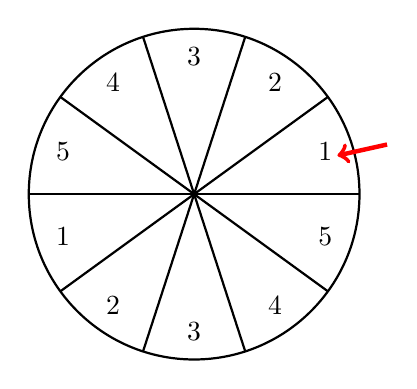
\begin{tikzpicture}[scale=.7]
        \foreach \i in {1,...,10} {
            \draw[thick] (0,0) -- ({36*\i}:3);
            %\node at ({30*(\i-0.5)}:2.5) {\i};
        }
        \foreach \i in {1,2,3,4,5} {
            \node at ({36*(\i-0.5)}:2.5) {\i};
            \node at ({36*(\i+4.5)}:2.5) {\i};
        }
        \draw[thick] (0,0) circle(3);
        \draw[->, ultra thick, red] (3.5,.9) -- (2.6,.7); % Ajout de la flèche
    \end{tikzpicture}
}
\begin{enumerate}
    \item Quelle est la loi de probabilité suivie par $X$ ?
    \item Combien de points un joueur peut-il espérer gagner en moyenne lors d'une partie ?
    \item Pour pouvoir tourner la roue, le joueur doit payer 1 euro. Un point rapporte 0,30 €. Le jeu est-il équitable?
\end{enumerate}

\textcolor{UGLiBlue}{\textbf{Correction}
\begin{enumerate}
    \item $X$ suit une loi uniforme sur $\{1,2,3,4,5\}$.
    \item L'espérance de $X$ est $\dfrac{1+2+3+4+5}{5}=3$. Un joueur peut donc espérer gagner 3 points en moyenne lors d'une partie.
    \item Le joueur doit payer 1 euro pour jouer. Il peut espérer gagner $3\times 0,3$ € soit 0,90 €. Le jeu n'est donc pas équitable.\\
\end{enumerate}}

%\vspace*{.5cm}


\dleft{13.5cm}{
    \exo{ Au casino}
    On suppose que la probabilité de gagner une partie à une machine à sous est de 0,001.\\
    On suppose que toutes les parties sont indépendantes et on appelle $X$ la variable aléatoire qui donne le rang de la première partie gagnée lorsqu'on joue plusieurs parties successives.\\
}
{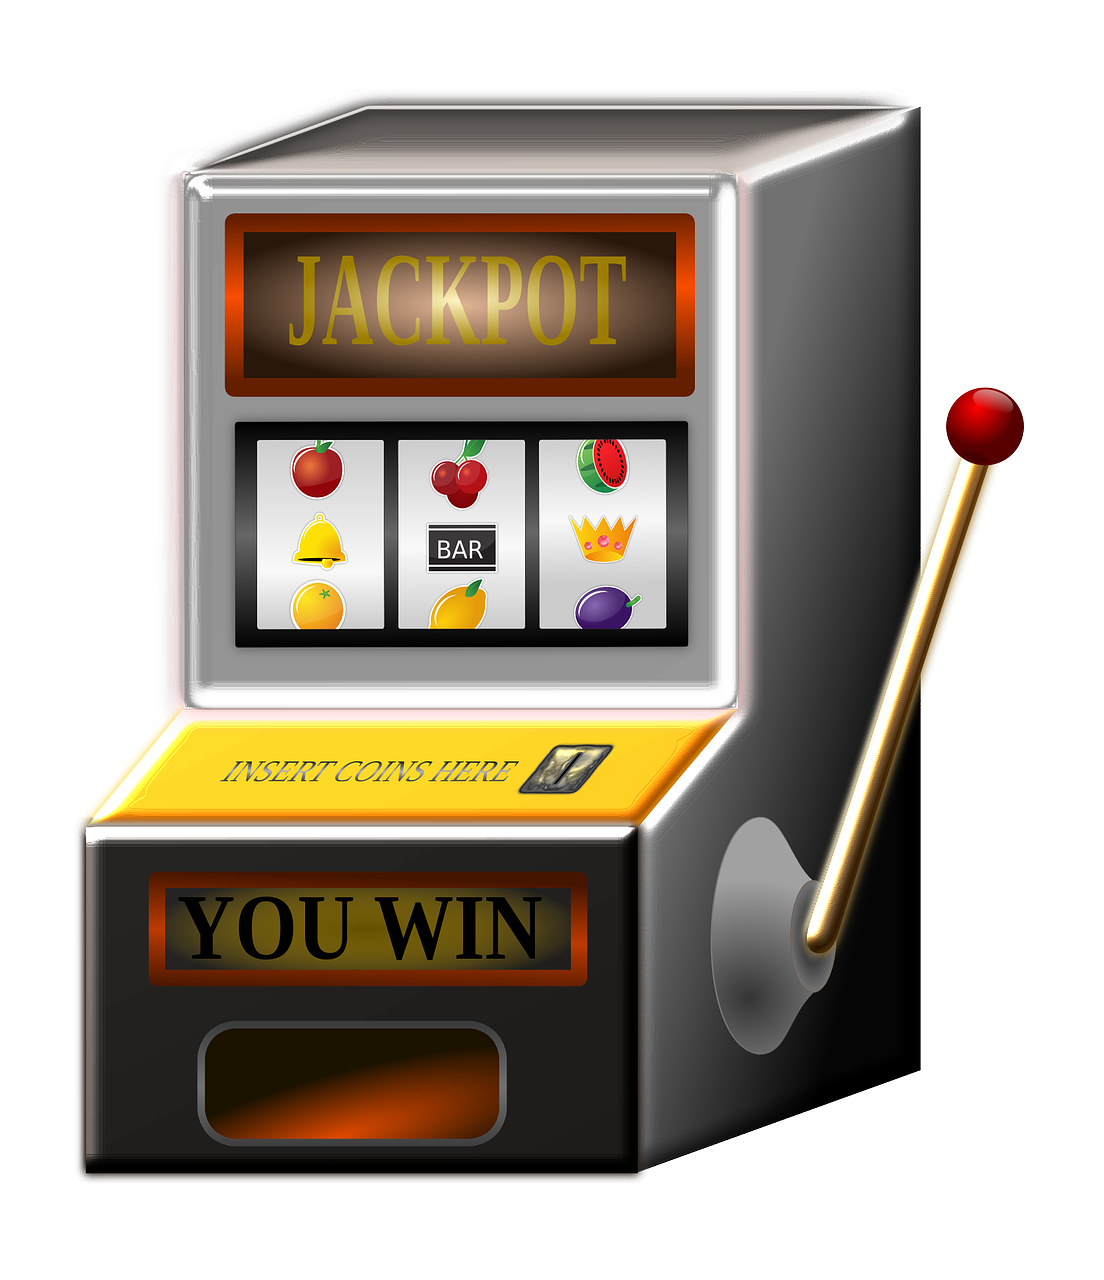
\includegraphics[width=3cm]{casino-161438_1280.png}}
\begin{enumerate}
    \item Quelle est la loi de probabilité suivie par $X$ ? Préciser le ou les paramètres.
    \item En combien de parties peut-on espérer gagner pour la première fois avec cette machine à sous ?
    \item Calculer $P(X>500)$ puis interpréter ce résultat.
    \item La mise de cette machine à sous est de 2 €.\\
    Quelle est la probabilité que l'on gagne avant de ne plus avoir d'argent si on dispose de 2000 € ?
\end{enumerate}

\textcolor{UGLiBlue}{\textbf{Correction}
\begin{enumerate}
    \item Cette expérience consiste à répéte une épreuve de Bernoulli de paramètre $p=0,001$.\\
    La variable aléatoire $X$ donne le nombre d'essais nécessaires pour obtenir le premier succès (gagner une partie) dans le schéma de Bernoulli de paramètre $p=0,001$.\\
    $X$ suit donc une loi géométrique de paramètre $p=0,001$.
    \item L'espérance de $X$ est $\dfrac{1}{0,001}=1000$. On peut donc espérer gagner pour la première fois en moyenne au bout de 1000 parties.
    \item $P(X>500)=(1-0,001)^{500}=0,999^{500}\approx 0,6064$.\\
    La probabilité de gagner pour la première fois après plus de 500 parties est d'environ 60,64\%.\\
    Autrement dit, la probabilité de ne pas gagner au cours des 500 premières parties est d'environ 60,64\%.
    \item On dispose de 2000 € qui permettent de jouer 1000 fois.\\
    La probabilité de gagner avant de ne plus avoir d'argent est $P(X\leqslant 1000)=1-P(X> 1000)=1-(1-0,001)^{1000}\approx 0,6321$.\\
    La probabilité de gagner avant de ne plus avoir d'argent si on dispose de 2000 € est d'environ 63,21\%.
\end{enumerate}}    


\dleft{11cm}{
    \exo{ Planche de Galton}
    Dans une fête foraine, on fait glisser un palet le long d'une planche cloutée comme ci-contre.\\
    À chaque étage, le palet rencontre un clou et va à gauche ou à droite avec la même probabilité. Après 4 étages, le palet arrive dans un des cinq bacs de réception numérotés de 0 à 4.}
{
    \begin{tikzpicture}
        % Dessiner les étages
        \foreach \i in {0,1,2,3} {
            \foreach \j in {0,...,\i} {
                \filldraw[black] (\j-\i/2, -\i) circle (2pt);
                % Ajouter des flèches à droite et à gauche de la bille
                \draw[->, thick] (0.1+\j-\i/2, -0.1-\i) -- (0.3+\j-\i/2, -0.5-\i);
                \draw[->, thick] (-0.1+\j-\i/2, -0.1-\i) -- (-0.3+\j-\i/2, -0.5-\i);
            }
        }
        
        % Dessiner les lignes de sortie
        \foreach \i in {-1,0,1,2,3,4} {
            \draw[thick] (\i-1.5, -3.5) -- (\i-1.5, -4.5);
        }
        \foreach \i in {0,1,2,3,4} {
            \node[UGLiBlue] at (\i-2,-4) {\i};
        }
        
        % Dessiner les bords de la planche
        \draw[thick] (-.5, 0.5) -- (-2.5, -3.5);
        \draw[thick] (.5, 0.5) -- (2.5, -3.5);
        \draw[thick] (-2.5, -4.5) -- (2.5, -4.5);
        
        % Ajouter une bille au sommet
        \filldraw[UGLiBlue] (0, 0.5) circle (5pt);
        
    \end{tikzpicture}
}
\begin{enumerate}
    \item \begin{enumalph}
        \item  Dans quel bac le palet arrivera-t-il s'il va à gauche puis à droite, puis à gauche, puis à gauche ?
        \item Dans quel bac le palet arrivera-t-il s'il va à droite puis à droite, puis à gauche, puis à droite ?
    \end{enumalph}
   \item On appelle $X$ la variable aléatoire qui donne le numéro du bac de réception du palet.
   \begin{enumalph}
        \item Expliquer pourquoi la loi de probabilité de $X$ est une loi binomiale dont on précisera les paramètres $n$ et $p$.
        \item Calculer l'espérance de $X$.
        \item Le gros lot est gagné si le palet arrive dans le bac 4.\\
        Quelle est la probabilité de gagner le gros lot ?
    \end{enumalph}
\end{enumerate}

\textcolor{UGLiBlue}{\textbf{Correction}
\begin{enumerate}
    \item \begin{enumalph}
        \item Le palet arrive dans le bac 1.
        \item Le palet arrive dans le bac 3.
    \end{enumalph}
    \item \begin{enumalph}
        \item À chaque clou rencontré, on considère que l'on obtient un succès si le palet va à droite et un échec s'il va à gauche.\\
        La variable aléatoire $X$ donne le nombre de succès dans une suite de $n=4$ épreuves de Bernoulli indépendantes de paramètre $p=\dfrac{1}{2}$.\\
        $X$ suit donc une loi binomiale de paramètres $n=4$ et $p=\dfrac{1}{2}$.
        \item L'espérance de $X$ est $np=4\times\dfrac{1}{2}=2$.
        \item La probabilité de gagner le gros lot est $P(X=4)=\displaystyle\binom{4}{4}\left(\dfrac{1}{2}\right)^4=\dfrac{1}{16}$.
    \end{enumalph}
\end{enumerate}}



\exo{ Loi de refroidissement de Newton}
Une tasse de café est servie à une température initiale de 80°C. On la laisse refroidir dans une pièce à température ambiante de 10°C.\\
On va étudier à l'aide d'une suite le refroidissement du café en appliquant la loi de Newton.\\

Pour tout entier naturel $n$, on note $t_n$ la température du café (en °C) au bout de $n$ minutes.\\
On a ainsi $t_0=80$. Entre deux minutes consécutives $n$ et $n+1$, on a $t_{n+1}-t_n=-0,2(t_n-10)$.
\begin{enumerate}
    \item Conjecturer d'après le contexte le sens de variation de la suite $(t_n)$.
    \item Montrer que, pour tout entier naturel $n$, on a $t_{n+1}=0,8t_n+2$.
    \item Exprimer $t_n$ en fonction de $n$.
    \item Déterminer la limite de la suite $(t_n)$.
    \item \faCalculator \hspace*{.2cm} Combien de temps faut-il pour que la température du café soit inférieure à 20°C ?
\end{enumerate}

\textcolor{UGLiBlue}{\textbf{Correction}
\begin{enumerate}
    \item On étudie le refroidissement d'un café. La température du café devrait donc diminuer et la suite $(t_n)$ devrait donc être décroissante.
    \item Soit $n$ un entier naturel.
    \begin{tabbing}
        $t_{n+1}$\=$=t_n-0,2(t_n-10)$\\
        \> $=t_n-0,2t_n+2$\\
        \> $=0,8t_n+2$.
    \end{tabbing}
    \item On a pour tout $n\in\N, t_{n+1}=0,8t_n+2$ et $t_0=80$.\\
    $(t_n)$ est une suite arithmétique de premier terme $t_0=80$ et de raison $q=0,8$.\\[.5em]
    \textbf{Suite constante vérifiant la relation de récurrence :} \begin{tabbing}
        Soit $x\in\R \qquad x=0,8x+2$\=$\iff x-0,8x=2$\\
        \>$\iff 0,2x=2$\\
        \>$\iff x=10$.
    \end{tabbing}
    La suite constante $(c_n)$ égale à 10 vérifie donc la relation $c_{n+1}=0,8c_n+2$ pour tout $n\in\N$.\\[.5em]
    \textbf{Suite géométrique auxiliaire :}\\[.5em]
    On définit la suite $(v_n)$ sur $\N$ par $v_n=t_n-c_n$.\\
    Montrons que $(v_n)$ est une suite géométrique :
    \begin{tabbing}
        Soit $n\in\N \qquad v_{n+1}$\=$=t_{n+1}-c_{n+1}$\\
        \> $=0,8t_n+2-(0,8c_n+2)$\\
        \> $=0,8t_n+2-0,8c_n-2$\\
        \> $=0,8(t_n-c_n)$\\
        \> $=0,8v_n$.
    \end{tabbing}
    $(v_n)$ est donc une suite géométrique de raison $q=0,8$ et de premier terme $v_0=t_0-c_0=80-10=70$.\\
    On a donc pour tout $n\in\N, v_n=v_0\times 0,8^n=70\times 0,8^n$.\\[.5em]
    \textbf{Terme général de la suite $(t_n)$ :}\\[.5em]
    On a donc pour tout $n\in\N, t_n=c_n+v_n=10+70\times 0,8^n$.
    \item $\lim\limits_{n\to+\infty}0,8^n=0$.\\[.5em]
    Donc $\lim\limits_{n\to+\infty} t_n=\lim\limits_{n\to+\infty}10+70\times 0,8^n=10$.\\[.5em]
    La température du café tend donc vers 10°C.
    \item On cherche le plus petit entier $n$ tel que $t_n<20$.\\
    On a $t_8\approx 21,7$ et $t_9\approx 19,4$.\\
    Il faut donc 9 minutes pour que la température du café soit inférieure à 20°C.
\end{enumerate}}
\end{document}